\jxhj{%教学后记
	}
\skrq{%授课日期
	2017年 | 4月11日 |4月18日|4月25日  | 1-3节}
\ktmq{%课题名称
	 椭圆加工	}
\jxmb{%教学目标,每行前面要加 \item
	\item 掌握宏程序的编程;
	\item 掌握宏程序加工椭圆的工艺;
	\item 巩固刀具半径补偿的灵活使用。}
\jxzd{%教学重点,每行前面要加 \item
	\item 宏程序的编程;
	\item 椭圆的工艺。}
\jxnd{%教学难点,每行前面要加 \item
	\item 宏程序的编程。}
\jjff{%教学方法
	通过讲述、举例、演示法来说明;}

\makeshouye %制作教案首页

%%%%教学内容
\subsection{实习教学要求}
\begin{enumerate}[\hspace{2em}1、]
	\item 掌握两面加工时的对刀;
	\item 掌握宏程序的编程;
	\item 掌握宏程序加工的工艺;
    \item 掌握两面加工时的精度控制;
\end{enumerate}

\subsection{相关工艺}
\subsubsection{编写椭圆程序}
加工如图\ref{椭圆加工}所示的零件。
\begin{figure}[!hbtp]
	\centering	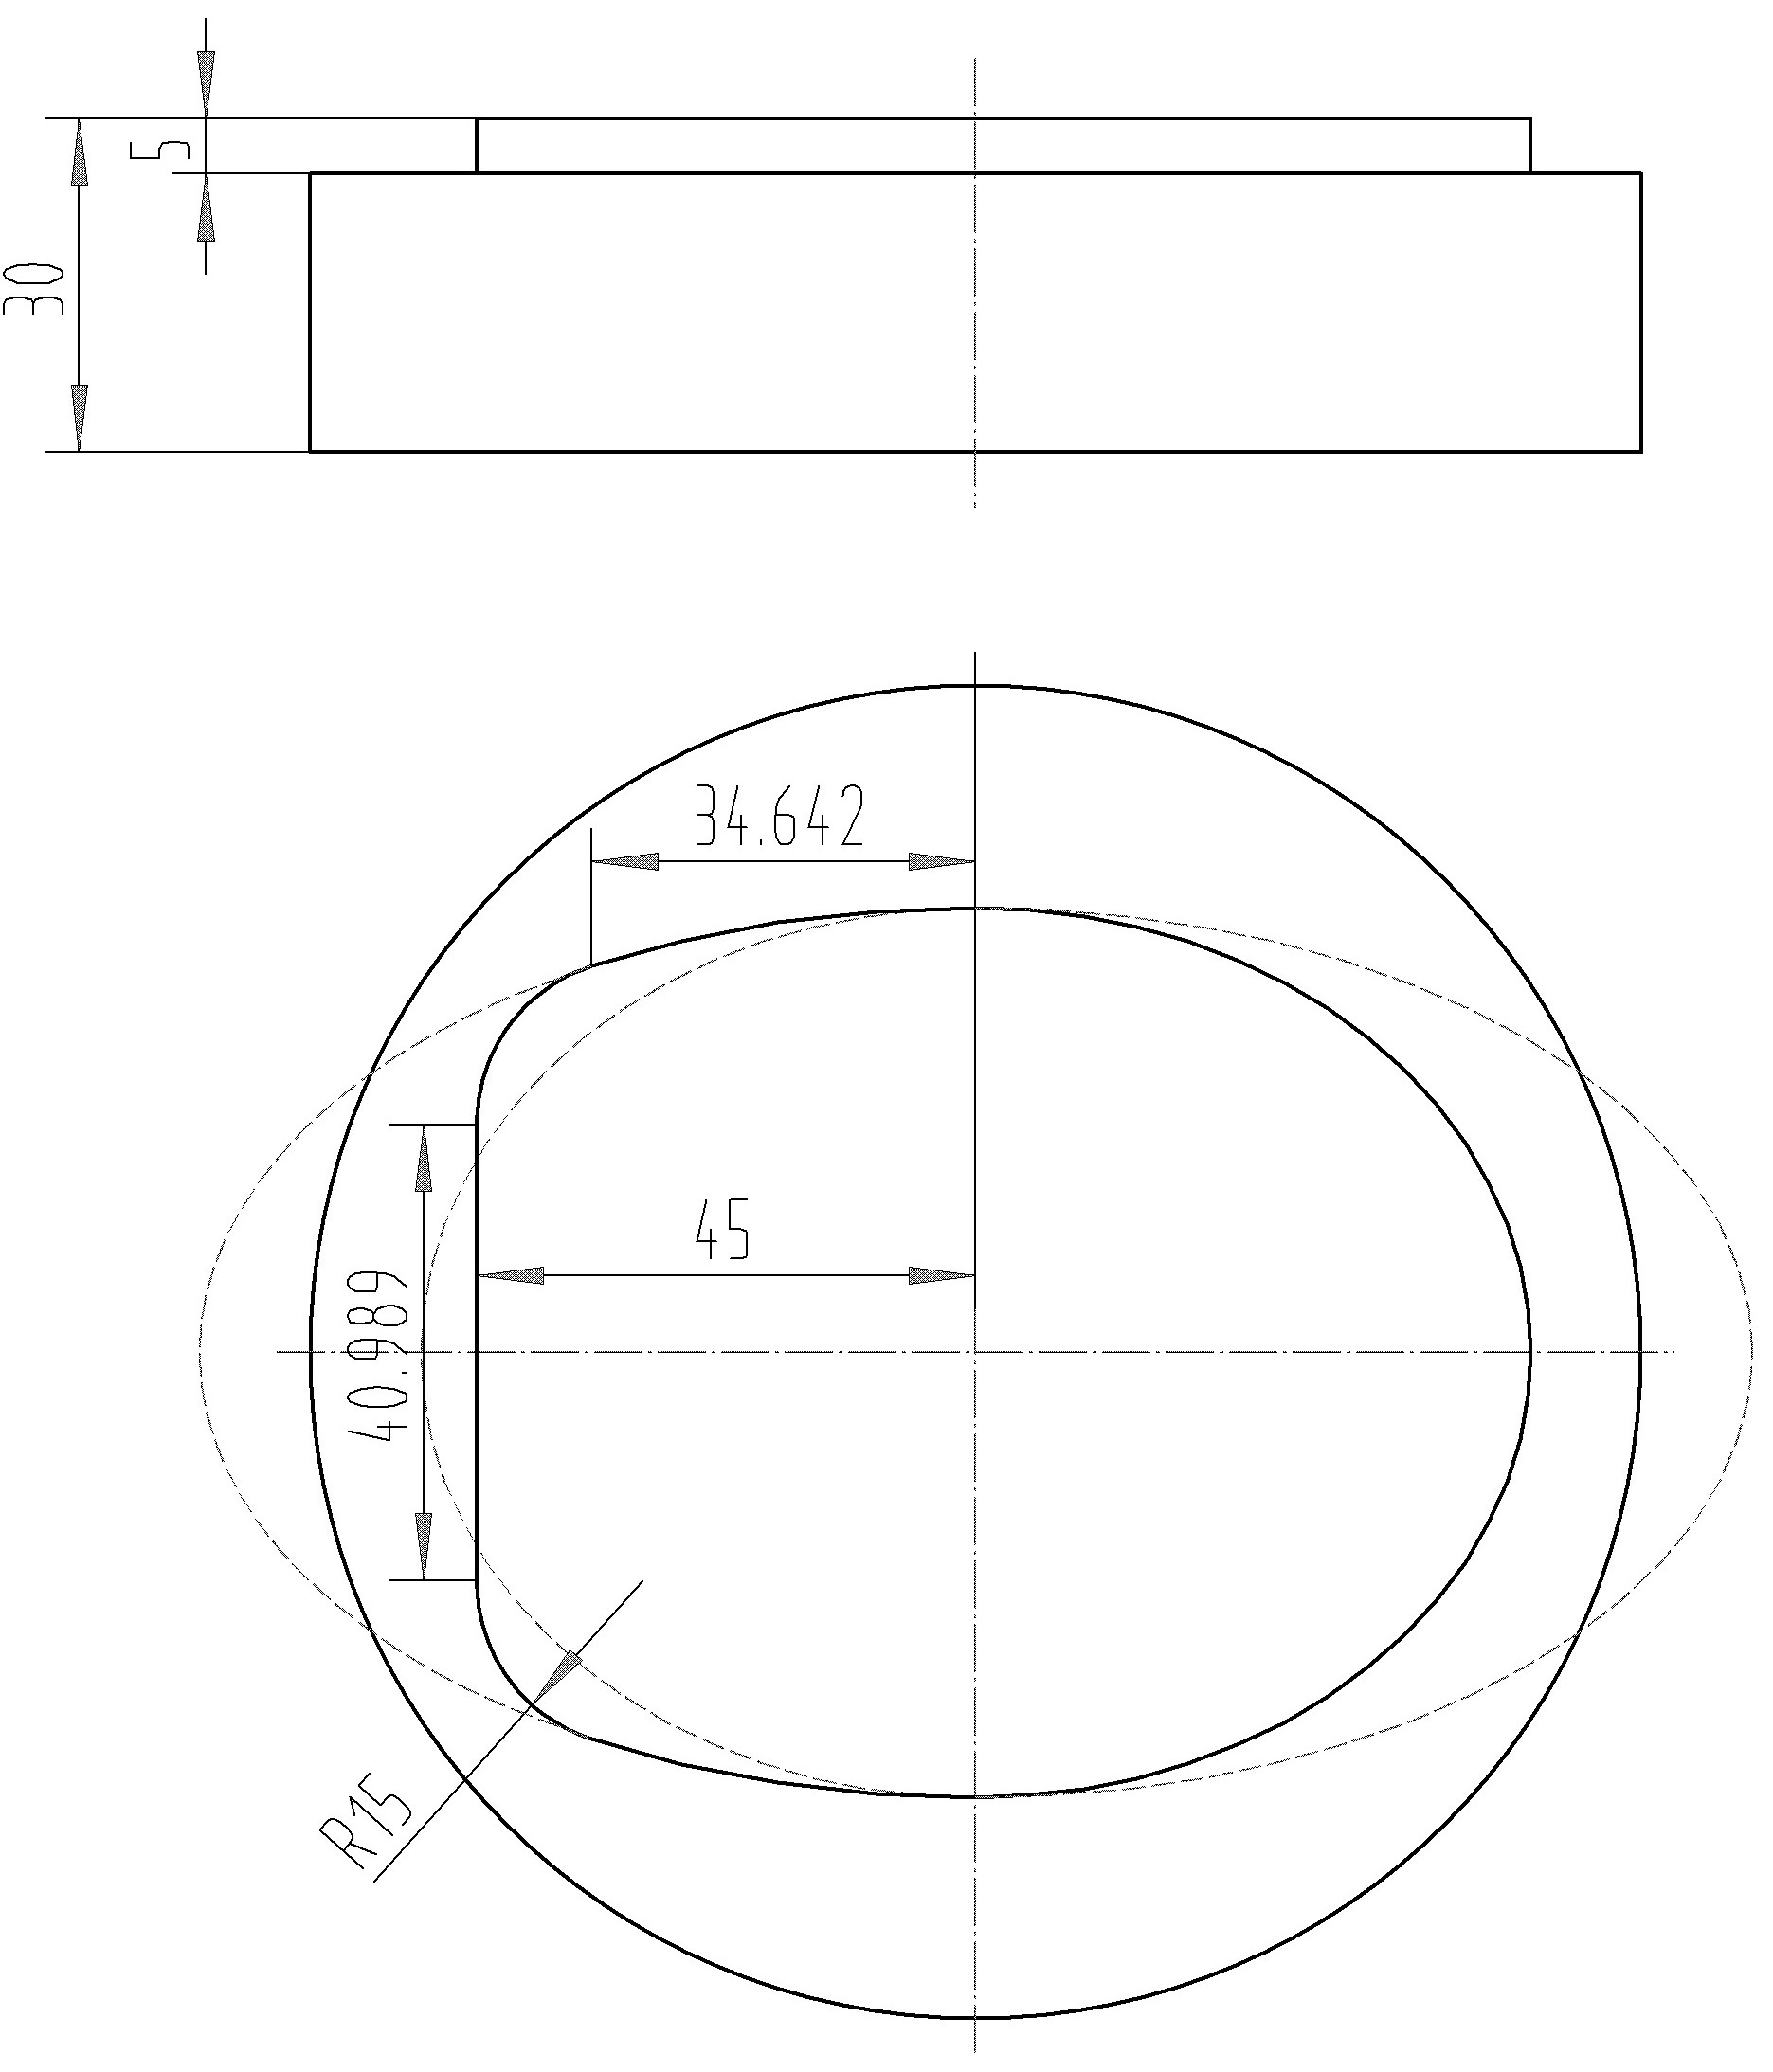
\includegraphics[width=0.6\textwidth]{images/shixi_1-1}
	\caption{椭圆加工} \label{椭圆加工}
\end{figure}

椭圆方程如下:
\[
\frac{x^2}{70^2}+\frac{y^2}{40^2}=1
\]
\[
\frac{x^2}{50^2}+\frac{y^2}{40^2}=1
\]

\begin{lstlisting}
GX01 
G54G17G40G90G64
CFTCP(关闭圆角半径修调)
T1D1
M3S500
G1Z30.F2000
X-70.Y0
Z5.0
Z-5.0F200
G1G41X-60.0Y-15.D1
G3X-45.Y0R15.
G1Y20.495
R1=ACOS(-34.642/70)
R2=-R1
G2 X-34.642  Y=40*SIN(R1)  CR=15.
WHILE  R1 >90
R1=R1-1
G1 X=70*COS(R1)  Y=40*SIN(R1)
ENDWHILE
WHILE  R1>-90
R1=R1-1
G1 X=50*COS(R1)  Y=40*SIN(R1)
ENDWHILE
WHILE  R1>R2
R1=R1-1
G1 X=70*COS(R1)  Y=40*SIN(R1)
ENDWHILE
G2 X-45. Y20.495 R15.
G1 Y0
G3X-60.Y15.R15.
G1G40X-70.Y0
Z30.F2000
M5
M2
\end{lstlisting}

\subsubsection{正弦曲线加工}
加工如图\ref{正弦曲线加工}所示的零件。
\begin{figure}[!hbtp]
	\centering	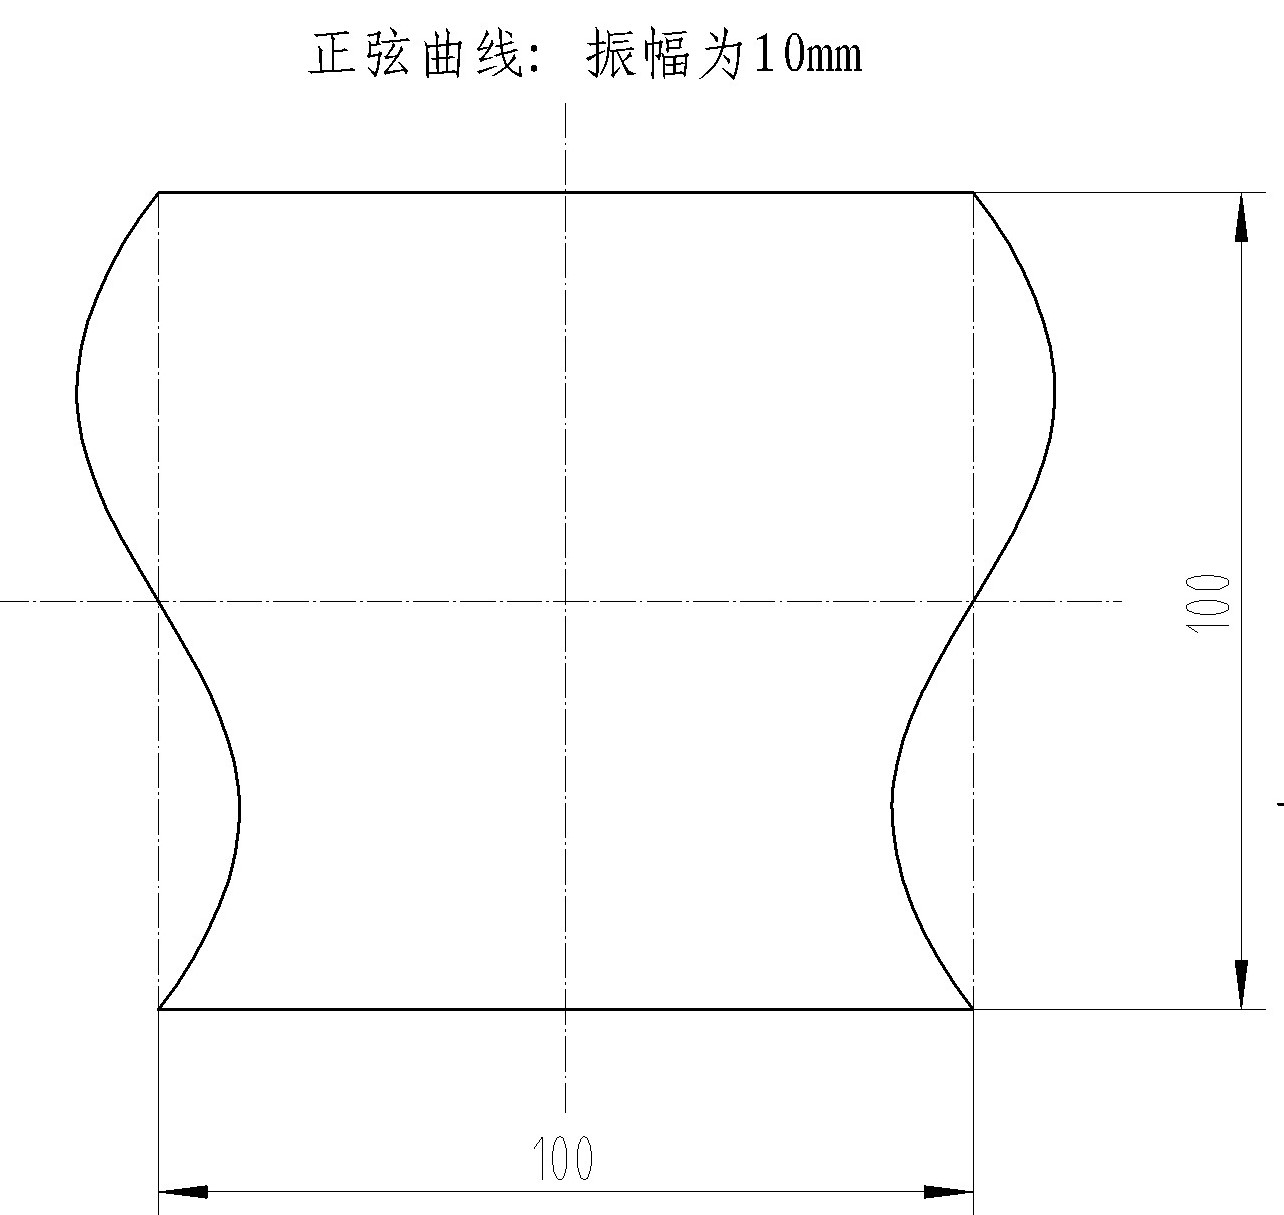
\includegraphics[width=0.6\textwidth]{images/shixi_1-2}
	\caption{正弦曲线加工} \label{正弦曲线加工}
\end{figure}

参考程序:
\begin{lstlisting}
GX02
G64G54G17G40G90CFTCP
T1D1
M3S500
G1Z30.F2000
X0 Y60.
Z5.0
Z-5.0F200
G41 X15.0 Y65. D1
G3X0 Y50.CR=15.
G1 X50. 
R1=50
MM1: R1=R1-0.5
G1 Y=R1 X=50+10*SIN(3.6*R1)
IF R1>-50 GOTOB MM1
G1X-50.
MM2: R1=R1+0.5
G1 Y=R1 X=-50+10*SIN(3.6*(R1+50))
IF R1<50 GOTOB MM2
G1X0
G3X15.0Y65.CR=15.
G1G40Y70.
Z30.F2000
M5
M2
\end{lstlisting}


\subsubsection{螺旋线}
(宏程序与极坐标的使用)

\subsubsection{切削用量}
有些宏程序加工的步距很小,可采用高的切削速度

如倒角

倒圆等



\subsection{实习内容及过程}

\subsubsection{集合、组织实习}
1、清查学生人数

2、文明安全生产讲解

3、实习内容说明
\subsubsection{开机15分钟}
1、由组长记录机床相关问题

2、开机前检查仔细

3、空转几分钟预热
\subsubsection{机床操作及编程}
1、教师演示基本操作

2、组长安排2人员操作机床(1人操作,1个指导)

3、其他人员自选图形编程

4、每人操作时间不得超过2小时

5、教师巡回指导
\subsubsection{操作点评及工件检测}
1、学生操作感想说明及自评

2、教师提问及点评

3、学生对工件自测

4、教师检测及评分
\subsubsection{准备下课}
1、清洁数控机床

2、正常关机

3、集合教师点评

\subsection{练习题及作业}
\begin{enumerate}[1、]
	\item 小结;
	\item 基本指令;
	\item 相关知识
	\item 机床操作
	\item 编程思路。
\end{enumerate}

\vfill
\subsection{加工准备与加工要求}
\subsubsection{加工准备}
\begin{enumerate}[1、]
\item 设备:数控铣床、加工中心。
\item 材料:45圆钢(Ф110*35)。
\item 工具:活动扳手,平行垫铁,百分表,其它常用辅具。
\item 量具:外径千分尺(0~25、100~125,0.01),深度千分尺(0~25,0.01),R规。
\item 刀具:Ф10、Ф16、Ф14立铣刀、Ф64面铣刀。
\item 夹具:三爪自定心卡盘、螺杆压板、平口钳。
\end{enumerate}
\subsubsection{课题评分表}

\noindent
\begin{figure}[!hbtp]
	\centering	
\begin{tabular}{|c|c|c|c|c|c|c|c|}
	\hline 
\multicolumn{2}{|c|}{工件编号}  &\multicolumn{2}{c}{} & \multicolumn{2}{|c|}{总得分}   & \multicolumn{2}{|c|}{ }   \\ 
	\hline 
 \multicolumn{2}{|c|}{项目与配分} &序号  & 技术要求 & 配分 & 评分标准 & 检测 记录  & 得分 \\ 
	\hline 
 工件加工 (80) &上面  & 1 &面铣  & 4 & 超差全扣 & & \\ 
	\hline 
 \multicolumn{2}{|c|}{} &  &  &  &  &  &  \\ 
	\hline 
\multicolumn{2}{|c|}{} &  &  &  &  &  &  \\ 
	\hline 
\end{tabular} 
\end{figure}


工件编号		总得分	
项目与配分	序号	技术要求	配分	评分标准	检测
记录	得分
工件
加工
(80%)		1	面铣	4	超差全扣		
2	尺寸1	12	超差全扣		
3	尺寸2	12	超差全扣		
4	椭圆	30	超差全扣		
程序与工艺
(10%)	10	程序正确合理	5	每错一处扣2分		
11	加工工序卡	5	不合理每处扣2分		
机床操作
(10%)	12	机床操作规范	5	出错一次扣2分		
13	工件刀具装夹	5	出错一次扣2分		
安全文明生产
(倒扣分)	14	安全操作	倒扣	安全事故停止操作或酌情扣分		
15	机床整理	倒扣			

\vfill